%%%%
%% Design :: Activity Diagrams
%%%
\section{Activity Diagrams}
\label{sec:activity_diagrams}

Within the \nameref{sec:primary_path} section a primary path analysis was 
conducted, ensuring that common paths throughout the proposed system are 
identified. Within this section a number of activity diagrams will be presented
that will break the primary path into a number of simple processes. 

An activity is a task in a process that allows for small meaningful work to 
happen. A process may have a number of activities linked together to form a work
flow \citep{lunn03}.

Figure \ref{fig:system_activity} on page \pageref{fig:system_activity},
illustrates the main activity diagram for the complete system. The activity
diagram follows what was discussed within the \nameref{sec:primary_path}
section, and expands upon some of the generalised points. Over the following
subsections key parts of the main activity diagram will be discussed in more
detail.

\begin{figure}[H]
  \centering
  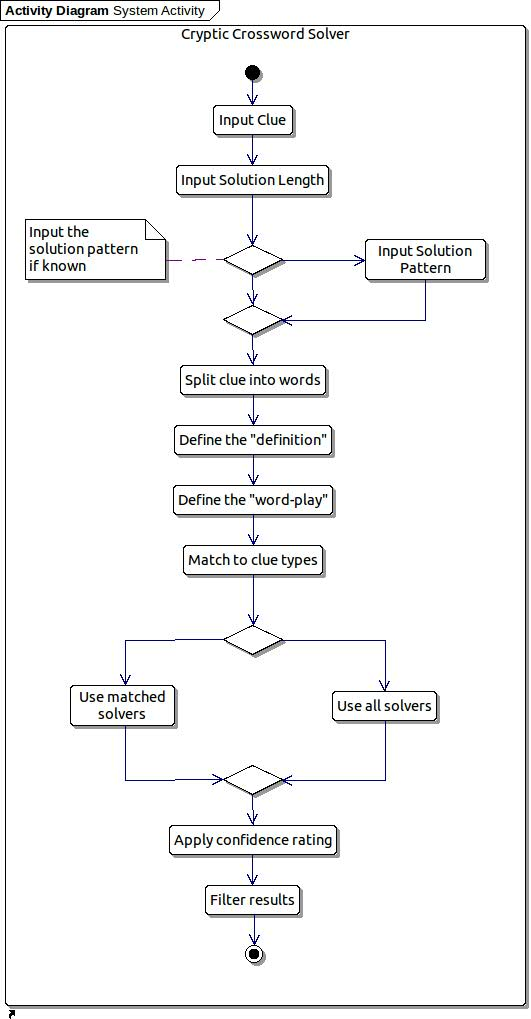
\includegraphics[scale=0.55]{activity/system_activity.jpg}
  \caption{The complete Activity diagram}
  \label{fig:system_activity}
\end{figure}


%%%
%%  Activity Diagram :: Handling Input
%%%
\subsection{Clue Input} 
\label{sub:input}

Figure \ref{fig:input_activity} illustrates how the data should be input into 
the system. In order for the system to solve a given clue it requires the 
following three inputs:

\begin{itemize}
  \item the clue 
  \item the solution length
  \item the solution pattern
\end{itemize}

At first it may seem that the solution length is unnecessary, as it could be 
computed from the solution pattern. The reason for including the solution length
is that it provides an additional validation element --- much like having to 
type in a password twice when creating a new online account.

The solution pattern allows a user to predefine the required answer, based upon 
a number of characters. The solution pattern will accept all letters as well as 
three predefined `special characters', as outlined below:

\begin{itemize}
  \item[] \textbf{?} $\Rightarrow$ wild card character
  \item[] \textbf{-} $\Rightarrow$ hyphenated word 
  \item[] \textbf{,} $\Rightarrow$ word separator
\end{itemize}

For example, the pattern ``'????e?-in-???'' could match to ``mother-in-law'' or 
``father-in-law'', just as ``??????? d?????'' could match to ``sitting ducks''.
As identified upon the activity path, a user may simply present the correct 
number of wild card characters to denote a unknown pattern.

\begin{figure}[H]
  \centering
  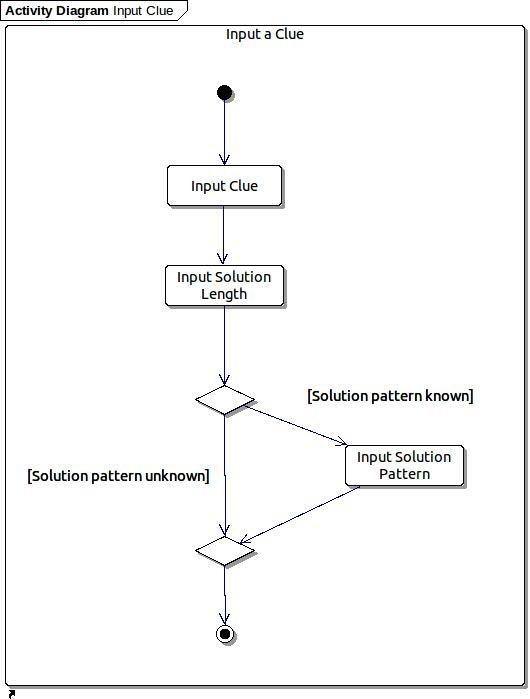
\includegraphics[scale=0.6]{activity/input_clue.jpg}
  \caption{Activity diagram showing how a user would input a clue}
  \label{fig:input_activity}
\end{figure}


%%%
%%  Activity Diagram :: Choosing a Solver
%%%
\subsection{Choosing a Solver} 
\label{sub:categorisation}

Once the user has successfully input the three variables, the system will then 
try to determine the type of clue. There are a number of actions that must be 
performed in order to deduce the type of clue, as shown in figure 
\ref{fig:categorisation_activity}.

The system will try to match the given clue to a list of properties that each 
clue has. For example spoonerism clue types, will have the word ``spooner''
within the clue.

If the match is successful then the system will bump the ranking of that 
particular clue type. Once the system has finished applying the categorisation 
`tests' to the clues, it will select the top solver to try to solve the clue.

If the chosen solver is unable to solve the clue, then the next ranking solver 
will try to solve. This process will continue until a set of results have been 
returned, or if all solvers have been used.

If the categorisation fails for some reason, then the system will try to brute 
force it's way to answer, by using all solvers.

\begin{figure}[H]
  \centering
  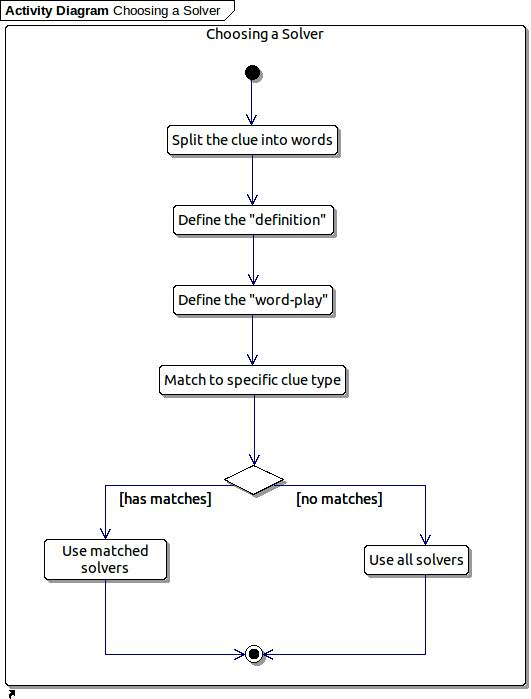
\includegraphics[scale=0.6]{activity/choosing_a_solver.jpg}
  \caption{Activity diagram showing how a solver is to be chosen}
  \label{fig:categorisation_activity}
\end{figure}


%%%
%%  Activity Diagram :: Handling Results
%%%
\subsection{Handling Results} 
\label{sub:results}

Once the solving process has finished, the system will then attempt to apply a 
`confidence rating'. The confidence rating of a clue is how close to the correct
answer the system thinks it is. 

For example, if a clue had a confidence rating of 100\% it would deemed as the 
only answer, whilst 0\% would indicate there is no chance of the answer being 
correct.

It is intended that if there are a large number of results, then the system may
choose to filter the results down. For example if thousands of results are 
generated, then the system may choose to only return results that have a 
confidence rating higher than 70\%.

Figure \ref{fig:results_activity} shows the handling of results as an activity 
diagram.

\begin{figure}[H]
  \centering
  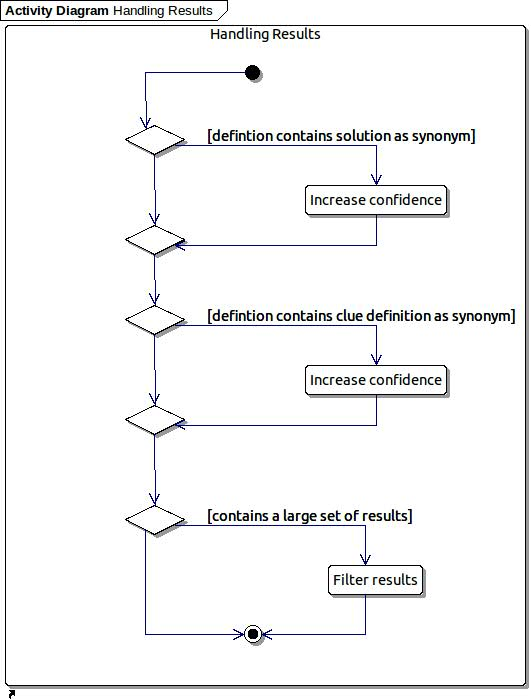
\includegraphics[scale=0.6]{activity/handling_results.jpg}
  \caption{Activity diagram showing how results should be handled}
  \label{fig:results_activity}
\end{figure}
